%%%%%%%%%%%%%%%%%%%%%%%%%%%%%%%%%%%%%%%%%
% Beamer Presentation
% LaTeX Template
% Version 1.0 (10/11/12)
%
% This template has been downloaded from:
% http://www.LaTeXTemplates.com
%
% License:
% CC BY-NC-SA 3.0 (http://creativecommons.org/licenses/by-nc-sa/3.0/)
%
%%%%%%%%%%%%%%%%%%%%%%%%%%%%%%%%%%%%%%%%%

%----------------------------------------------------------------------------------------
%	PACKAGES AND THEMES
%----------------------------------------------------------------------------------------

\documentclass{beamer}

\mode<presentation> {

% The Beamer class comes with a number of default slide themes
% which change the colors and layouts of slides. Below this is a list
% of all the themes, uncomment each in turn to see what they look like.

%\usetheme{default}
%\usetheme{AnnArbor}
%\usetheme{Antibes}
%\usetheme{Bergen}
%\usetheme{Berkeley}
%\usetheme{Berlin}
%\usetheme{Boadilla}
%\usetheme{CambridgeUS}
%\usetheme{Copenhagen}
%\usetheme{Darmstadt}
%\usetheme{Dresden}
%\usetheme{Frankfurt}
%\usetheme{Goettingen}
%\usetheme{Hannover}
%\usetheme{Ilmenau}
%\usetheme{JuanLesPins}
%\usetheme{Luebeck}
%\usetheme{Madrid}
%\usetheme{Malmoe}
%\usetheme{Marburg}
%\usetheme{Montpellier}
%\usetheme{PaloAlto}
%\usetheme{Pittsburgh}
%\usetheme{Rochester}
%\usetheme{Singapore}
%\usetheme{Szeged}
%\usetheme{Warsaw}

% As well as themes, the Beamer class has a number of color themes
% for any slide theme. Uncomment each of these in turn to see how it
% changes the colors of your current slide theme.

%\usecolortheme{albatross}
%\usecolortheme{beaver}
%\usecolortheme{beetle}
%\usecolortheme{crane}
%\usecolortheme{dolphin}
%\usecolortheme{dove}
%\usecolortheme{fly}
%\usecolortheme{lily}
%\usecolortheme{orchid}
%\usecolortheme{rose}
%\usecolortheme{seagull}
%\usecolortheme{seahorse}
%\usecolortheme{whale}
%\usecolortheme{wolverine}

%\setbeamertemplate{footline} % To remove the footer line in all slides uncomment this line
%\setbeamertemplate{footline}[page number] % To replace the footer line in all slides with a simple slide count uncomment this line

%\setbeamertemplate{navigation symbols}{} % To remove the navigation symbols from the bottom of all slides uncomment this line
}

\usepackage{graphicx} % Allows including images
\usepackage{booktabs} % Allows the use of \toprule, \midrule and \bottomrule in tables
\usepackage{datetime}

%----------------------------------------------------------------------------------------
%	TITLE PAGE
%----------------------------------------------------------------------------------------

\title[]{Optimising compiler from OCaml to WebAssembly} % The short title appears at the bottom of every slide, the full title is only on the title page

\author{Douglas Boyle} % Your name
\date{\formatdate{16}{2}{2021}} % Date, can be changed to a custom date

\begin{document}

\begin{frame}
\titlepage % Print the title page as the first slide
\end{frame}


%----------------------------------------------------------------------------------------
%	PRESENTATION SLIDES
%----------------------------------------------------------------------------------------

\begin{frame}\frametitle{Overview} 
\includegraphics[scale=0.37]{overview}
\begin{itemize}
\item Compiler for integer and basic floating point operations
\item Benchmark programs in OCaml, Grain and C
\item Compared against Js\_of\_ocaml, Grain and Clang/LLVM
\item All success criteria met
\end{itemize}
\end{frame}

\begin{frame}[fragile]  \frametitle{Intermediate Representation}
\begin{itemize}
\item Compiles patterns into IR code that performs pattern matching and variable binding

\begin{columns}[c] % The "c" option specifies centered vertical alignment while the "t" option is used for top vertical alignment
\column{.4\textwidth} % Left column and width
\begin{verbatim}
match x with
   | (1, y) -> y
   | _ -> 0

\end{verbatim}

\column{.4\textwidth} % Right column and width
\begin{verbatim}
let v0 = x.(0) in
  if v0 = 1
  then x.(1)
  else 0
\end{verbatim}
\end{columns} % If there were other cases, these would be checked instead at this point
\text{} \\
\text{} \\

\item Linearises code to simplify later stages % A-normal form

\begin{columns}[c] 
\column{.4\textwidth} 
\begin{verbatim}
f(g(x), h(y))


\end{verbatim}
\column{.4\textwidth} 
\begin{verbatim}
let v0 = g(x) in
  let v1 = h(y) in 
    f(v0, v1)
\end{verbatim}
\end{columns}
\end{itemize}
%Every argument to an operation is a variable name or constant.
\end{frame}

% TODO: Plot in matlab instead
% TODO: Rotate labels
%\begin{frame}\frametitle{Data Collected}
% Different benchmarks span an order of magnitude in execution time, so results are given as fraction of Js_of_ocaml's performance
% In every case Grain was an order of magnitude slower than Javascript
%\includegraphics[scale=0.33]{times_vs_js}
% Different benchmarks vary significantly in size, so given as fractino of Grain's filesize
%\includegraphics[scale=0.27]{filesize_vs_grain}

% Can see that my compiler outputs smaller files than both the JavaScript and Grain outputs. It is expected to be smaller than the Js_of_ocaml tool's output since WebAssembly has a binary format whereas JavaScript files are text. 
% Also outperforms both Grain and Js_of_ocaml in terms of execution speed. In each benchmark, Grain was about an order of magnitude slower than the output from Js_of_ocaml. This is not so surprising since my compiler does not implement garbage collection, whereas both the Grain and Js_of_ocaml programs will be garbage collected
%\end{frame}

\begin{frame}\frametitle{Evaluation}
\vspace{-1cm}
\begin{figure}
    \hspace*{-0.3in}
    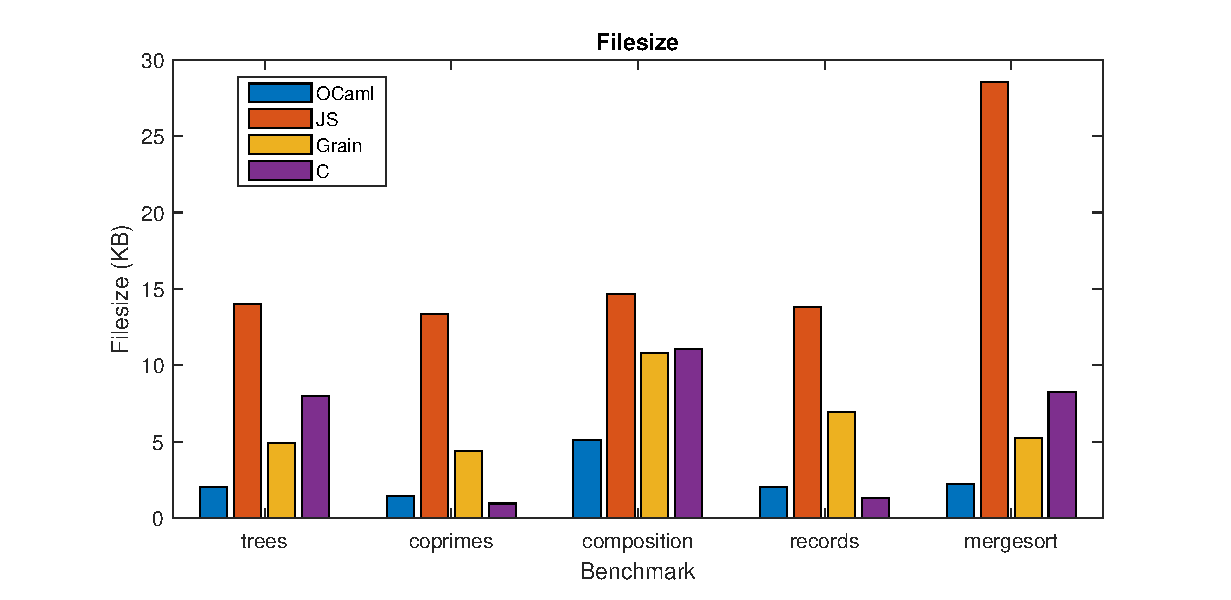
\includegraphics[scale=0.6]{filesize2}
\end{figure}
\vspace{-0.5cm}
\begin{itemize}
\item Execution time
\item Filesize
\item Heap usage
%\item Measured execution time, heap usage and output file size.
%\item Compiled code runs faster than both Grain and Js\_of\_ocaml output, likely due to there being no garbage collection.
\end{itemize}
\end{frame}

\begin{frame}\frametitle{Extensions} 
Language Extensions
\begin{itemize}
\item Floating point and reference operations
\end{itemize}
\text{} \\
Optimisations
\begin{itemize}
\item Inlining % With some heuristics based on other compilers, allows further optimisations to be detected
\item Tail Call Optimisation % For both functions recursive on their own and mutually recursive
\item Common Subexpression Elimination % Avoid recalculating immutable values that already exist
\item Dead Assignment Elimination % Allows compilation of pattern matching to introduce unnecessary assignments that are later removed
\end{itemize}
\text{}\\
Garbage Collection
\begin{itemize}
\item Initially by reference counting and later changed to tracing
\end{itemize}
\end{frame}


%%%%%%%%%%%%%%%%%%%%%%%%%%%%%%%%%%%%%%%%%%%%%%%%%%%%%%%%%%%%%%%%%%%%%%%%%%
\iffalse 

Slide 1: My project was to write a compiler from OCaml to WebAssembly and evaluate its performance compared to alternative compilers to WebAssembly.
Here we have an overview of the structure of my compiler. I took the parser and type-checker from the front end of the OCaml compiler, then compiled the output of this into my own intermediate representation. % Describe IR in more detail on next slide
From this I generate WebAssembly code, and I have also written a runtime system primarily in WebAssembly, but with garbage collection implemented in JavaScript.
Rather than supporting the full OCaml language, I decided to leave out the object and module layer, as well as many of the standard library operations except for integer and some floating point operations. This has given me more time to focus on optimisations.
After writing the compiler, I wrote a set of benchmark programs in OCaml, Grain and C and compiled each of these to WebAssembly to compare the performance of my compiler. 
% Mention in slide 3: I also compiled the OCaml programs to JavaScript using the Js\_of\_ocaml tool as another comparison for executing code in a browser.

Slide 2: My intermediate representation is based on the Lambda representation the OCaml compiler uses in later stages and the intermediate representation used by Grain. As with the Lambda language, it compiles OCaml's patterns into simpler code which matches those patterns, however many of the primitive operations in Lambda were not necessary due to the subset of OCaml being supported. Another difference to the Lambda representation is that code is linearised, so that each operation is just on constants or other variables, with the exception of control flow structures such as loops or function definitions. This simplifies analysis and later compilation, similar to using Continuation Passing Style, but is generally easier to translate to than the CPS terms.

Slide 3: I compared my compiler against Clang and LLVM for C code and also the Grain compiler,  two ways of compiling to WebAssembly. Additionally, I compiled each OCaml benchmark with Js_of_ocaml to get a JavaScript file that could also be run in the browser.
I have compared each of these methods in terms of the execution time, file size and heap usage of the resulting programs. Here we have the output filesizes for 5 different benchmarks. As you can see, the output of my compiler is consistently smaller than that of Grain and significantly smaller than converting the OCaml program to JavaScript. 
It is also smaller than the same program implemented in C and compiled with Clang, in the cases where the standard library is needed for memory allocation.
% Worth mentioning next bit or not?
Currently, there appears to be very limited support for importing the C library functions at runtime using WebAssembly's module interface, hence the disparity in filesize for the C examples.

Slide 4: Lastly, I have had time to implement several extensions to my project. First, I extended the operations and types supported by my compiler to allow floats and references. This was relatively straightforward but allows me to test a much wider range of benchmark programs focused on floating point calculations or imperative style code.
I have also added several optimisations, primarily at the intermediate representation. This includes the inlining of function calls and optimising both recursive and mutually recursive tail calls to help reduce the stack size used by function calls.
Within each procedure, there are optimisations to detect and avoid recomputing the same expression in multiple places, as well as removing variables which are never used. Inlining one function body inside another increases the number of opportunities found for doing this.
Finally, over the last few weeks I have implemented a garbage collector. In order to efficiently collect cyclic data structures, this uses a simple mark and sweep algorithm. In WebAssembly, stack frames and local variables aren't accessible through the linear memory, so this requires designating a region of memory to keep a shadow stack of all local variables in use, which is scanned to identify all reachable objects during garbage collection.

Over the next few weeks I intend to optimise parts of my Garbage Collector and collect additional data on the impact my optimisations have before I start writing the dissertation.

\fi
%----------------------------------------------------------------------------------------




\end{document} 